%%%============================================================================
%
%   Pandoc template to convert to latex using emulateapj.
%   
%
%   Usage:
%   ------
%
%   pandoc --template=[/Path/To/File/]pandoc-apj.latex
%
%
%
%   Caveats (mostly limitations in pandoc):
%   ---------------------------------------
%
%   + Doesn't do figure* and table* environments, these must be tweaked 
%     manually from standard figure and table environments or inserted as raw
%     LaTeX rather than Markdown figure invironments.
%     UPDATE: This can be accomplished by using Scholdoc rather than Pandoc.
%   + Same goes for equations: pandoc (at the time of writing) only does
%     displaymath, equations must be declared in raw LaTeX
%   + Graphics are not scaled, because the autoscale function provided in the
%     template is using the raw TeX \def function, which is not supported in
%     ApJ. UPDATE: This has been fixed in Pandoc, and Scholdoc even better.
%     Use Scholdoc! 
%
%   Copyright 2014-2016 T. E. Rivera-Thorsen.
%
%%%============================================================================
\documentclass[preprint2]{aastex6}
% \usepackage{lmodern}
% \usepackage{dcolumn}
\usepackage{amssymb,amsmath}
\usepackage[T1]{fontenc}
\usepackage[utf8x]{inputenc}
% \usepackage{natbib}
\bibliographystyle{aasjournal}
\usepackage{listings}
\usepackage{graphicx}
%\ifxetex
%  \usepackage[setpagesize=false, % page size defined by xetex
%              unicode=false, % unicode breaks when used with xetex
%              xetex]{hyperref}
%\else
%\usepackage[unicode=true]{hyperref}
%\fi
\hypersetup{breaklinks=true,
           bookmarks=true,
           pdfauthor={},
           pdftitle={Neutral ISM, Lyman-Alpha and Lyman-continuum in nearby starburst Haro 11},
           colorlinks=true,
           citecolor=blue,
           urlcolor=blue,
           linkcolor=magenta,
           pdfborder={0 0 0}}
\urlstyle{same}  % don't use monospace font for urls
% \setlength{\parindent}{0pt}
% \setlength{\parskip}{6pt plus 2pt minus 1pt}
% \setlength{\emergencystretch}{3em}  % prevent overfull lines
% \setcounter{secnumdepth}{5}

\shorttitle{Neutral ISM, Ly-Alpha and LyC in Haro 11}

\shortauthors{T. E. Rivera-Thorsen et al.}





% % \date{\today}
% 

%%%-----------------------------------------------------------------------
%      Macros
%%%-----------------------------------------------------------------------

\begin{document}

\title{Neutral ISM, Lyman-Alpha and Lyman-continuum in nearby starburst Haro 11\footnotemark[1]}
\footnotetext[1]{Based on observations Cosmic Origins Spectrograph on the Hubble Space
Telescope, program XXXXXX, PI YYYYYYYY}

\author{T. Emil Rivera-Thorsen\altaffilmark{2, 3}}

\author{Göran Östlin\altaffilmark{2, 3}}


\altaffiltext{2}{Department of Astronomy, Oskar Klein Centre, Stockholm University,
AlbaNova University Centre, SE-106 91 Stockholm, Sweden}
\altaffiltext{3}{Oscar Klein Centre for Cosmoparticle Physics, Department of Astronomy,
Stockholm University, Stockholm, Sweden}

\begin{abstract}
Something something something.
\end{abstract}

\section{Introduction and
Observations}\label{introduction-and-observations}

About Haro 11: Some of the same stuff as in Rivera-Thorsen et al. (in
prep.) could be mentioned, with a different emphasis. Star formation
rate should be mentioned from \citet{Adamo2010}. Population from same
and from \citet{Micheva2010}. Knots named by \citet{Vader1993}, and also
mentioned by \citet{Kunth2003}. It's an LBA \citep{Hoopes2007}, and an
LAE analog \citep{Hayes2007, Leitet2011}. Knot C a strong Ly$\alpha$
emitter \citep{Hayes2007}, and also a LyC emleaker
{[}\citet{Bergvall2006}; Leitet2011{]}. Kinematics, it's a merger
\citep{Ostlin1999, Ostlin2001, Ostlin2015}. More weight on the
Lyman-$\alpha$ escape thing, and LyC. Mention Ly$\alpha$ escape and the
histrory here, too? References:

\begin{figure*}
\centering
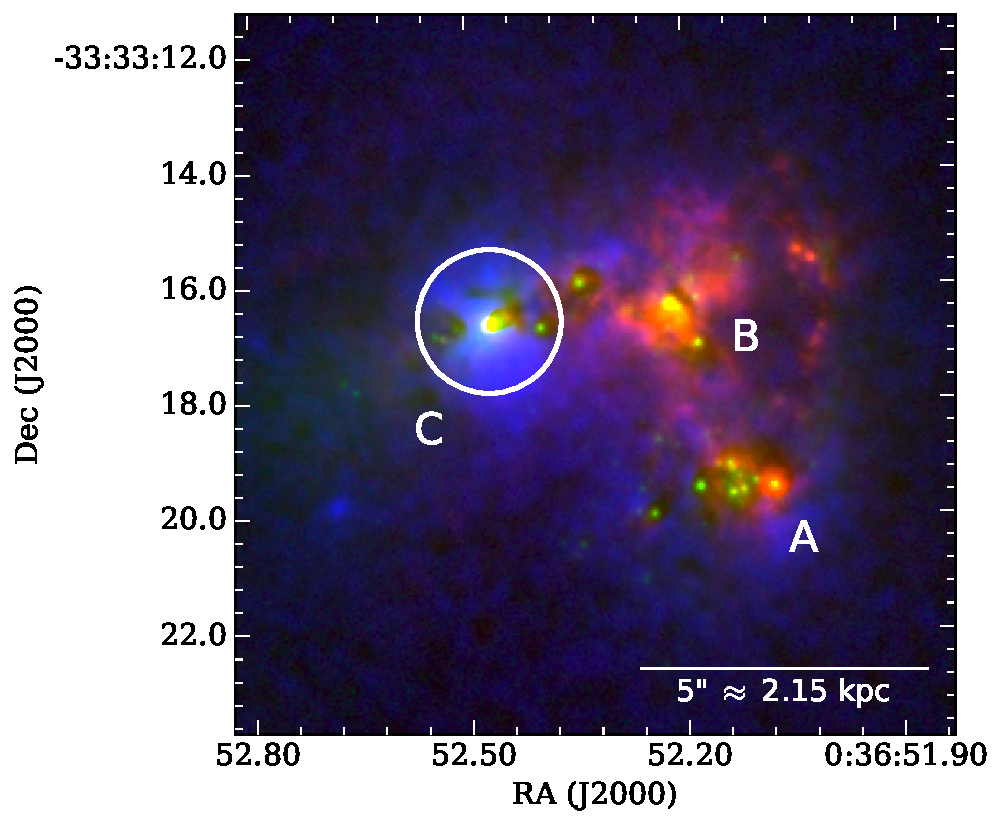
\includegraphics[width=0.600\hsize]{../Figs/Haroslit.pdf}
\caption{Approximate coverage of the COS aperture. The aperture, which
was centered on the supercluster in knot C, has a diameter of 2.5
\arcsec}\label{fig:apmap}
\end{figure*}

\begin{figure*}
\centering
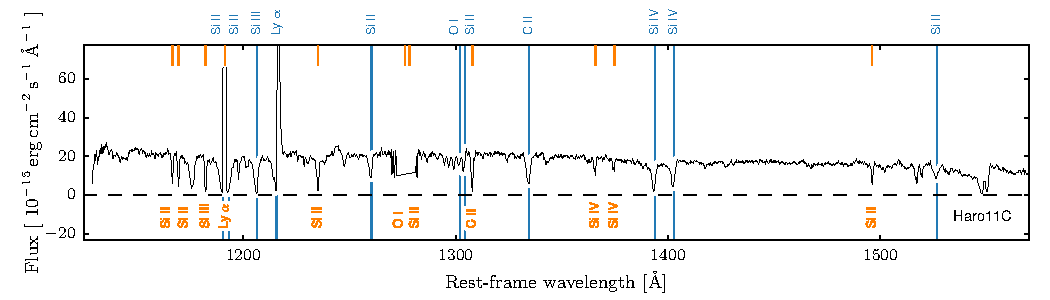
\includegraphics[]{../Figs/FullSpec.pdf}
\caption{Full spectrum in restframe wavelength of Haro 11 C. Redshift
adopted from \citet{Sandberg2013}. Orange lines denote Milky Way
absorption, while blue lines denote absorption internal to the
target.}\label{fig:fullspec}
\end{figure*}

\section{Analysis}\label{analysis}

\begin{figure}
\centering
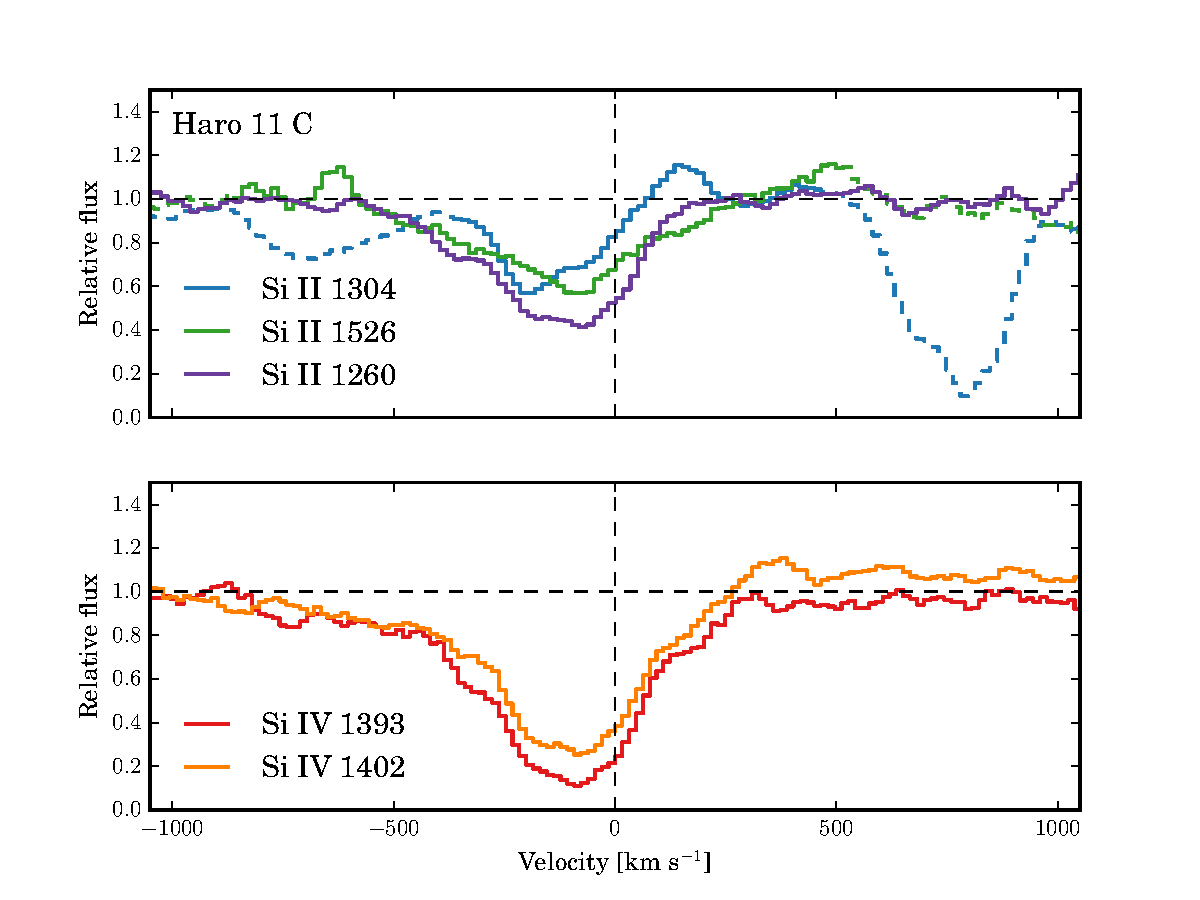
\includegraphics[width=3.500in]{../Figs/HISLISProfiles.pdf}
\caption{The \ion{Si}{2} (\textbf{upper}) and \ion{Si}{4}
(\textbf{lower}) profiles included in this
study.}\label{fig:SingleLines}
\end{figure}

\begin{figure}
\centering
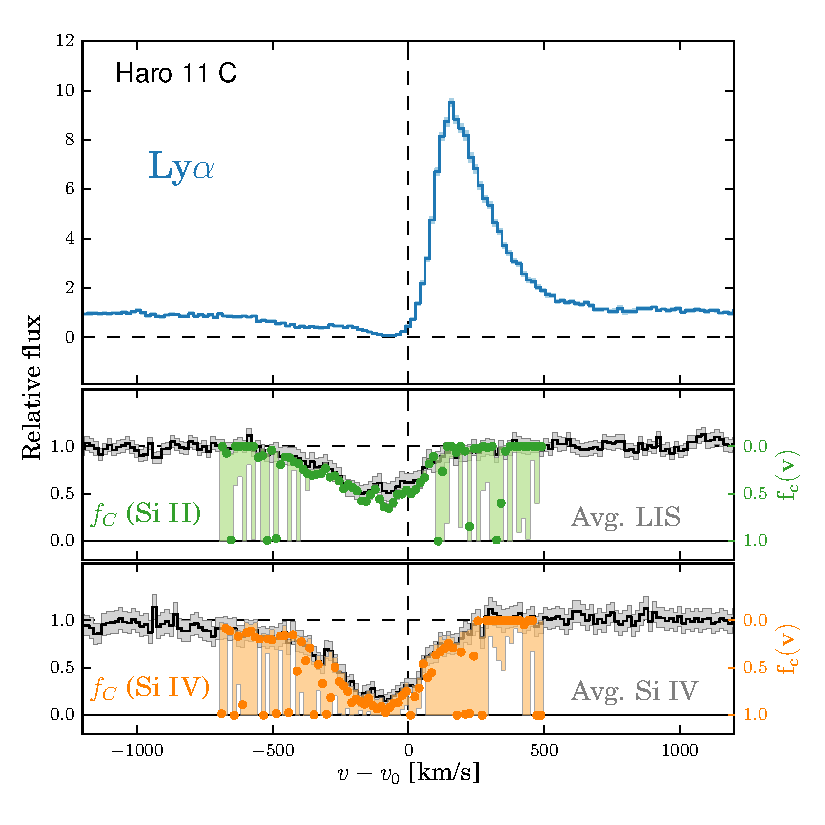
\includegraphics[width=3.500in]{../Figs/LyACoverfracs.pdf}
\caption{\textbf{Upper panel}: Ly$\alpha$ profile of Haro 11 C, in
approximate units of the surrounding continuum level. Full line is the
measured values smoothed by a 5 px. flat kernel; surrounding shading
encloses the $\pm 1 \sigma$ error band. \textbf{Middle panel}: Black
steps show the averaged, LIS line profile, smoothed by a 5px kernel.
Surrounding gray shading denotes the $\pm 1 \sigma$ confidence band.
\textbf{Lower panel}: Same as middle panel, but for the \ion{Si}{4}
transitions.}\label{fig:HisLisLya}
\end{figure}

Bla bla bla

\section{Discussion and conclusions}\label{discussion-and-conclusions}

Bla bla bla

\bibliography{./main.bib}

\end{document}
